% ============================================================================
% Chapter 2: Literature Review
% ============================================================================

\chapter{Literature Review}
\label{chap:literature}

This chapter reviews the state-of-the-art in swarm robotics, examining existing architectures, mechanical design approaches, and control strategies that inform the development of the AUSRA system.

\section{Evolution of Material Handling: From AGVs to AMRs}
\label{sec:agv_vs_amr}

\begin{figure}[H]
    \centering
    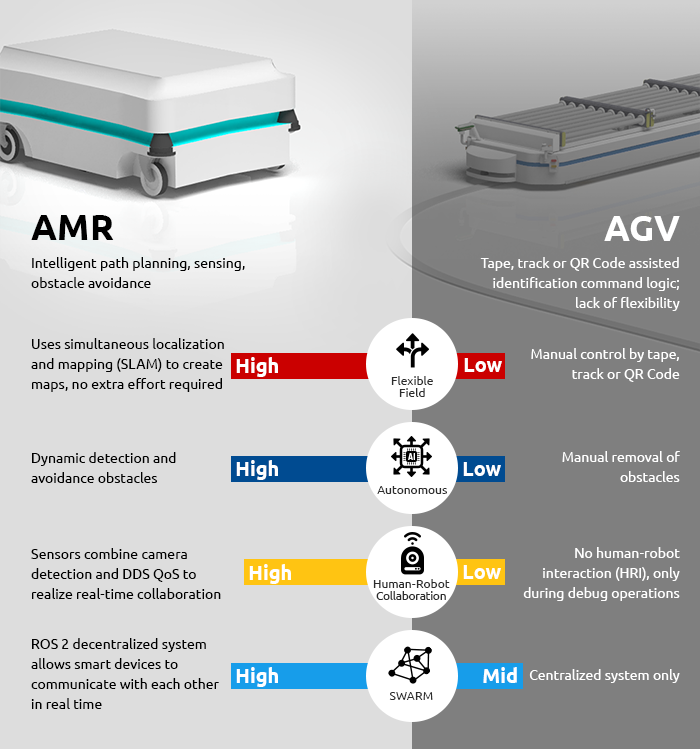
\includegraphics[width=0.6\linewidth]{figures/Chapter 2/AMRvsAGR.png}
    \caption{Evolution from AGVs to AMRs}
    \label{fig:amr_vs_agv}
\end{figure}

The coordination of mobile robots in industrial environments has evolved significantly, marked by a paradigm shift from Automated Guided Vehicles (AGVs) to Autonomous Mobile Robots (AMRs). This transition is driven by the increasing demand for flexibility and scalability in Industry 4.0 applications.

\subsection{The Limitations of AGVs}
Automated Guided Vehicles have been the standard for material transport for decades. However, they rely fundamentally on fixed infrastructure, such as magnetic tape, inductive wires, or visual markers on the floor. This dependency creates several critical limitations:
\begin{itemize}
    \item \textbf{Rigidity:} Modifying a robot's path requires physical alteration of the facility, leading to costly downtime.
    \item \textbf{Lack of Intelligence:} AGVs typically follow a "stop-and-wait" protocol when encountering obstacles. They cannot replan their path locally, which often leads to deadlocks in dynamic environments.
    \item \textbf{Installation Cost:} The need for facility modifications increases the initial deployment cost and time.
\end{itemize}

\subsection{The Superiority of AMRs}
Autonomous Mobile Robots represent the next generation of intelligent logistics. Unlike AGVs, AMRs utilize onboard sensors (Lidar, cameras) and Simultaneous Localization and Mapping (SLAM) algorithms to navigate without external infrastructure. The industry trend is heavily favoring AMRs due to their superior adaptability:
\begin{itemize}
    \item \textbf{Dynamic Navigation:} AMRs can detect obstacles and autonomously compute alternative paths in real-time, maintaining high throughput in cluttered environments.
    \item \textbf{Rapid Deployment:} A facility can be mapped digitally in hours rather than days, allowing for immediate operation.
    \item \textbf{Swarm Scalability:} New agents can be added to the fleet seamlessly by sharing the existing global map, making AMRs the ideal platform for swarm robotics research.
\end{itemize}

\begin{table}[H]
\centering
\caption{Comparative Analysis: AGV vs. AMR}
\label{tab:agv_vs_amr}
\begin{tabular}{|l|p{5cm}|p{5cm}|}
\hline
\textbf{Feature} & \textbf{Automated Guided Vehicle (AGV)} & \textbf{Autonomous Mobile Robot (AMR)} \\
\hline
\textbf{Navigation} & Physical guides (wires, tape, QR codes) & LiDAR, SLAM, Natural Features \\
\hline
\textbf{Flexibility} & Low (Requires infrastructure changes) & High (Software-defined paths) \\
\hline
\textbf{Obstacles} & Stops and waits until cleared & Navigates around dynamically \\
\hline
\textbf{Deployment} & Slow, disruptive installation & Fast, minimal facility impact \\
\hline
\textbf{Cost Model} & High initial infrastructure cost & Higher per-unit robot cost, but lower total ownership cost due to flexibility \\
\hline
\end{tabular}
\end{table}

\section{Existing Swarm Architectures}
\label{sec:swarm_architectures}

Swarm robotics has been an active research area since the early 2000s. Several notable systems and architectures have been developed:

\subsection{Kilobot}
The Kilobot platform, developed at Harvard University \cite{rubenstein2012kilobot} (Figure \ref{fig:kilobot}), is designed for large-scale swarm experiments. Key features include:
\begin{itemize}
    \item Low-cost design (approximately \$14 per unit)
    \item Infrared communication for local messaging
    \item Vibration motors for differential drive locomotion
    \item Collective charging capabilities
\end{itemize}

\subsection{e-puck}
The e-puck \cite{mondada2009puck} (Figure \ref{fig:epuck}) is a widely used educational and research platform featuring:
\begin{itemize}
    \item Differential drive with stepper motors
    \item Multiple sensor modalities (camera, IR, accelerometer)
    \item Open-source hardware and software
\end{itemize}

\subsection{Industrial Solutions}
Commercial swarm robotics systems have emerged in warehouse automation:
\begin{itemize}
    \item \textbf{Amazon Robotics (Kiva):} Grid-based navigation with centralized coordination (Figure \ref{fig:kiva})
    \item \textbf{Geek+:} Autonomous mobile robots for goods-to-person systems (Figure \ref{fig:geekplus})
    \item \textbf{Locus Robotics:} Collaborative picking robots with decentralized control (Figure \ref{fig:locus})
\end{itemize}

% Add comparison table here
\begin{table}[H]
\centering
\caption{Comparison of Existing Swarm Platforms}
\label{tab:swarm_comparison}
\begin{tabular}{|l|c|c|c|c|}
\hline
\textbf{Platform} & \textbf{Cost} & \textbf{Locomotion} & \textbf{Communication} & \textbf{Autonomy} \\
\hline
Kilobot & Very Low & Vibration & IR & Limited \\
e-puck & Medium & Differential & Bluetooth/IR & Moderate \\
Kiva & High & Differential & WiFi & High \\
AUSRA & Medium & Omnidirectional & WiFi/ROS & High \\
\hline
\end{tabular}
\end{table}

% Add detailed content here...

\begin{figure}[H]
    \centering
    % Row 1: Kilobot, E-puck, Amazon Kiva
    \begin{subfigure}[b]{0.3\textwidth}
        \centering
        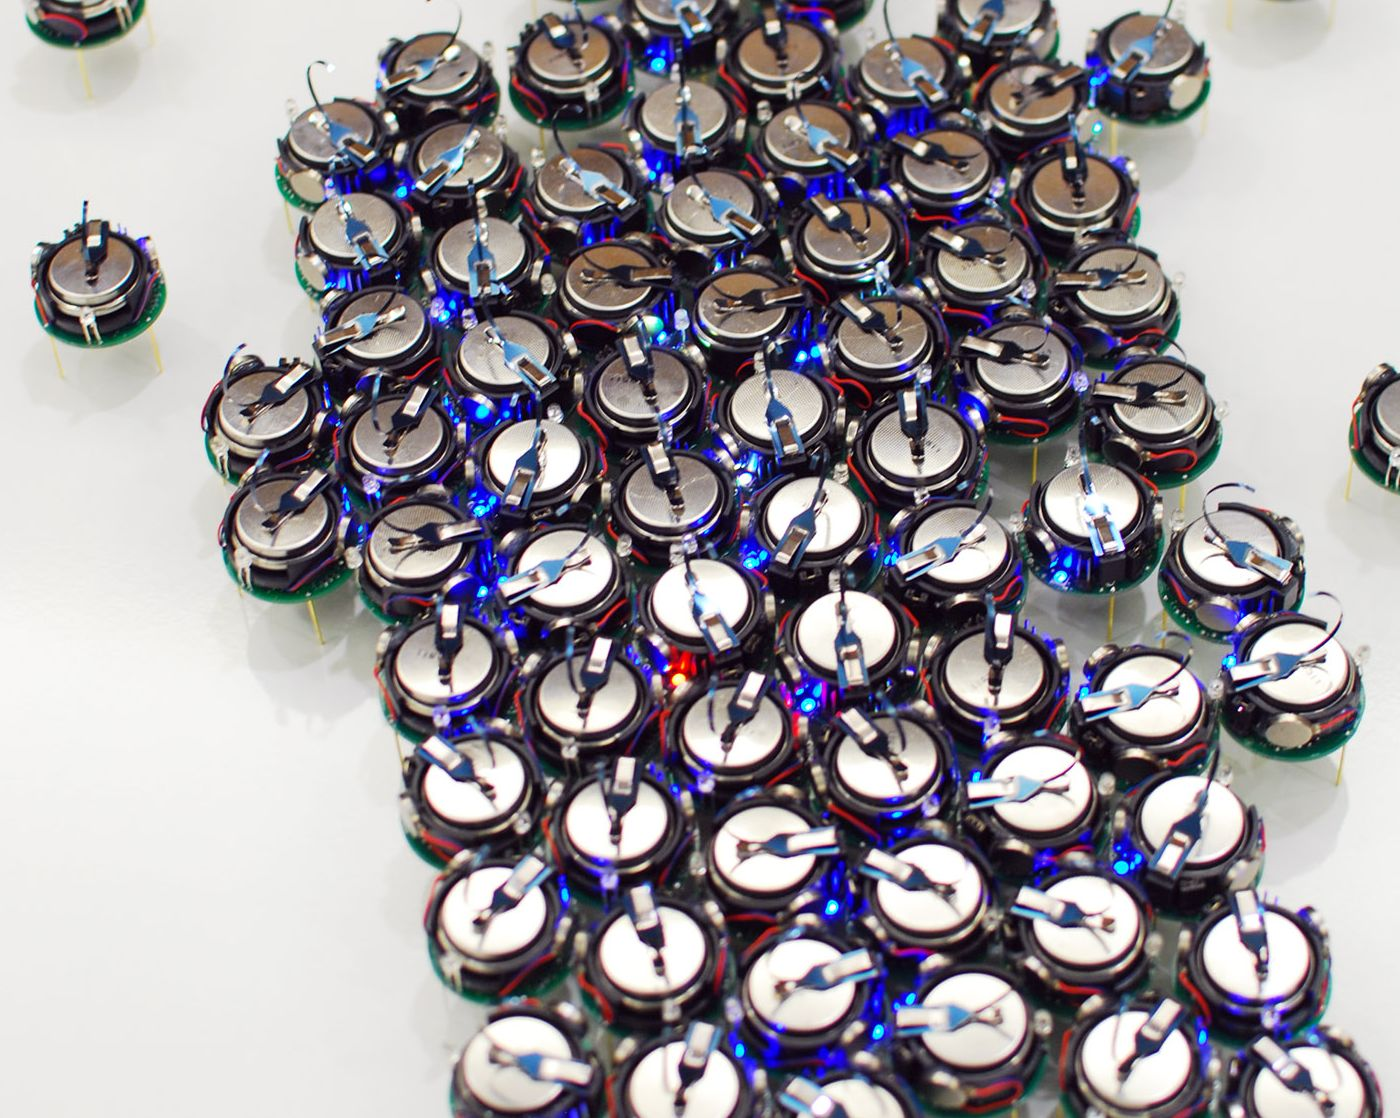
\includegraphics[width=\linewidth]{figures/Chapter 2/Kilo_bots.jpg}
        \caption{Kilobots}
        \label{fig:kilobot}
    \end{subfigure}
    \hfill
    \begin{subfigure}[b]{0.3\textwidth}
        \centering
        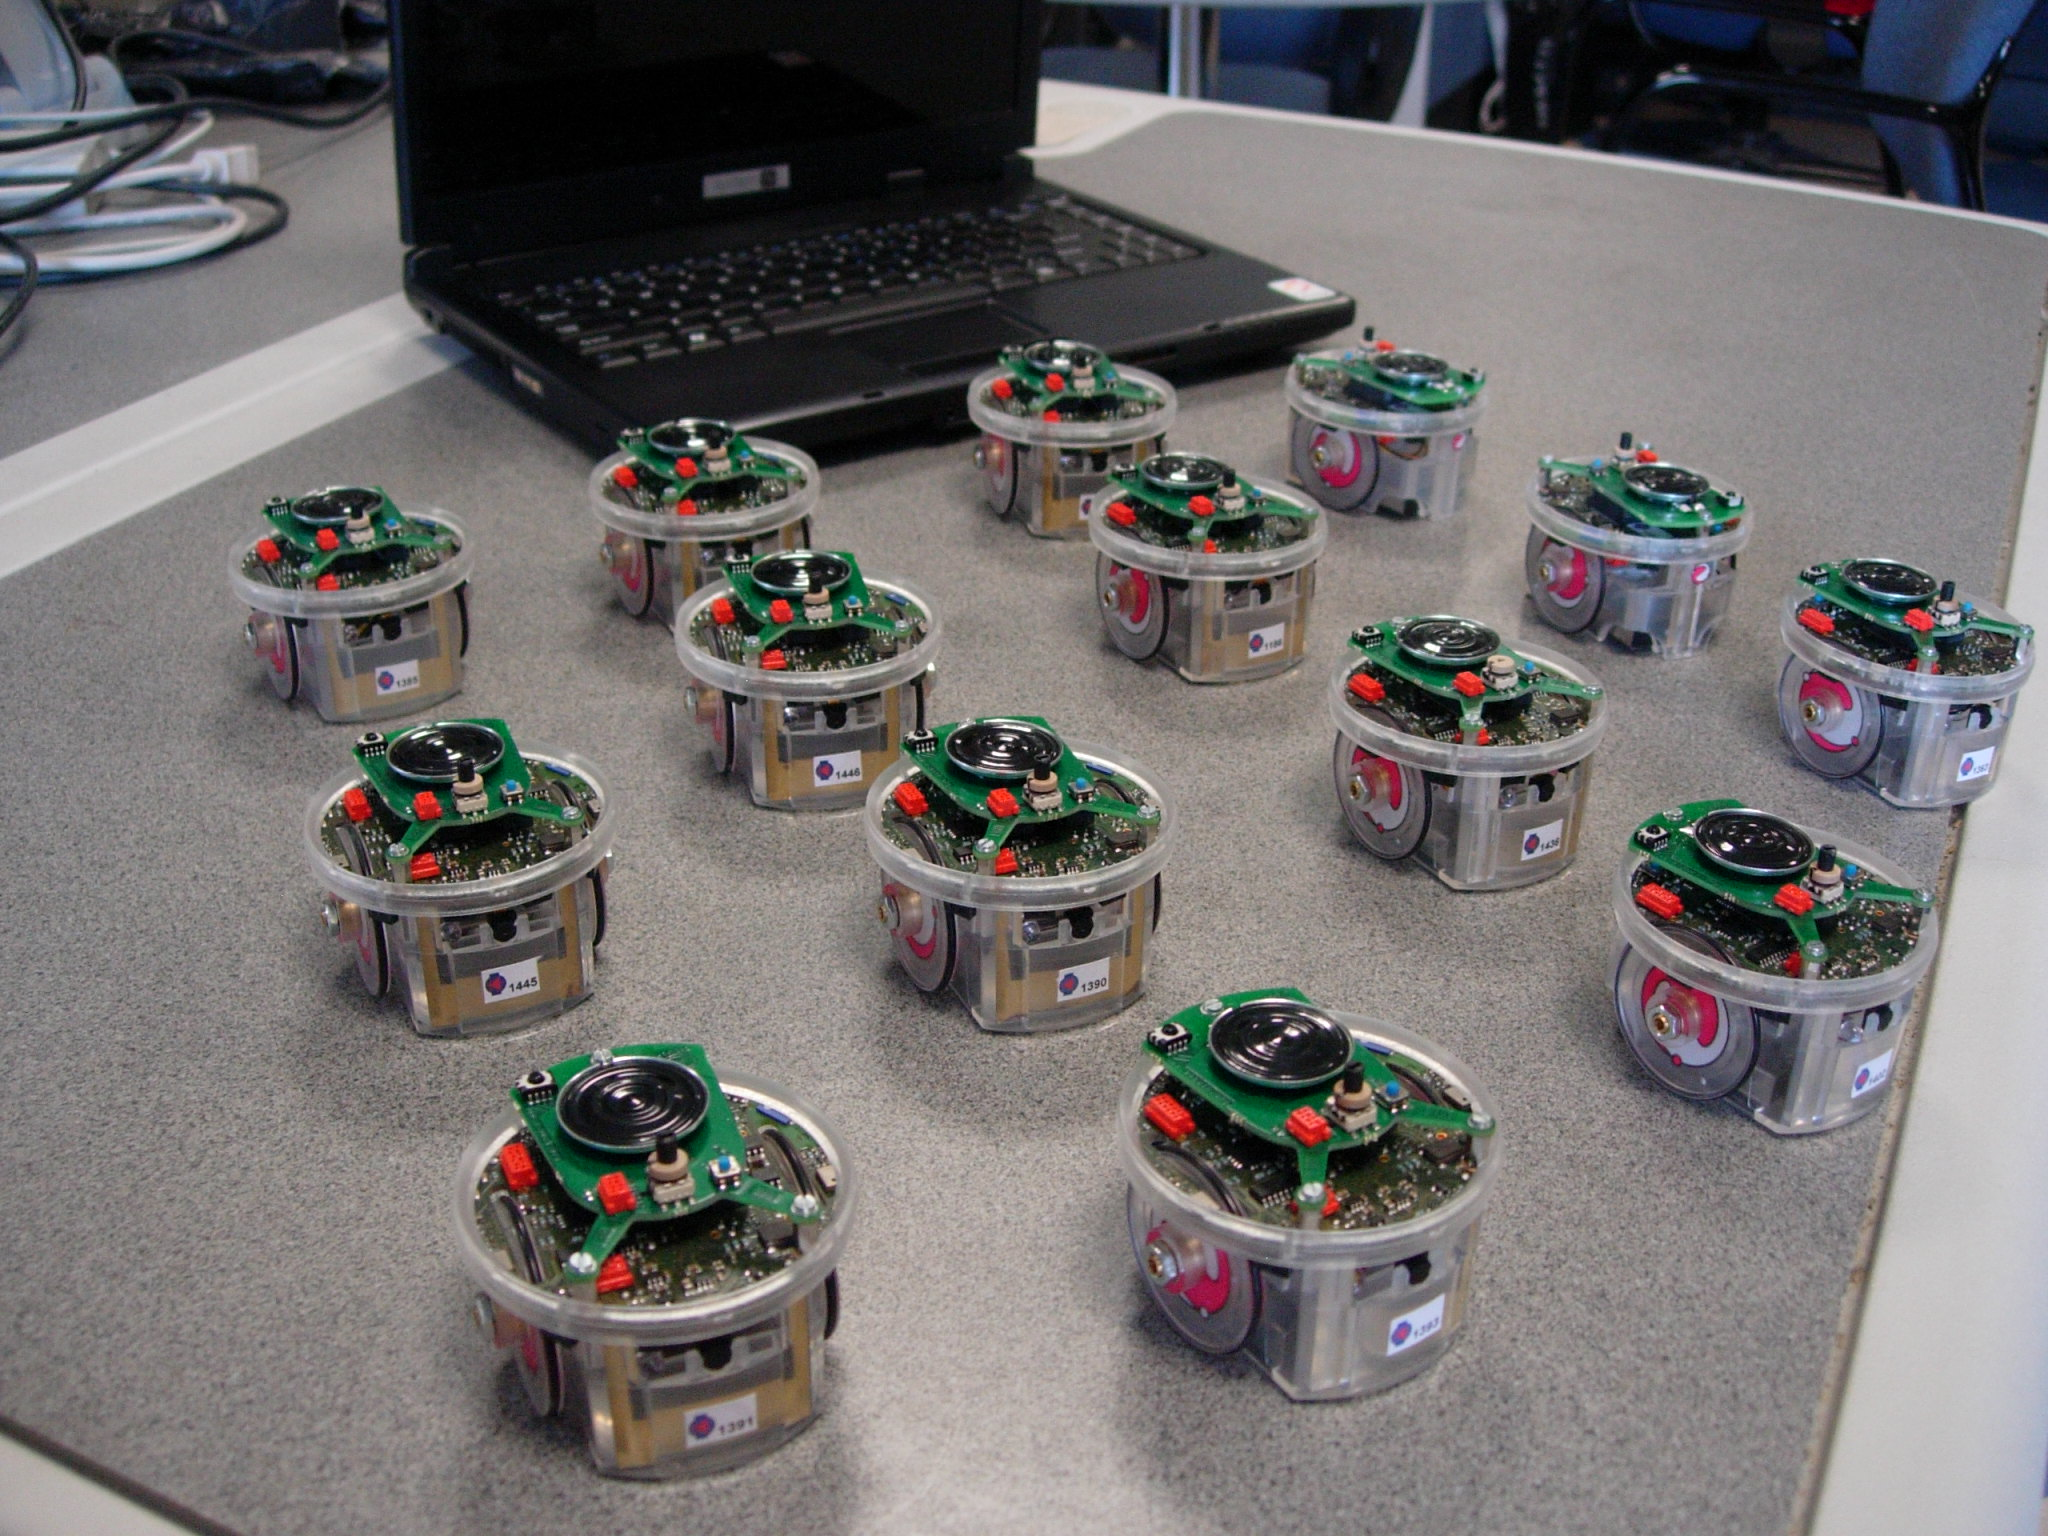
\includegraphics[width=\linewidth]{figures/Chapter 2/E-puck_robots.png}
        \caption{E-puck}
        \label{fig:epuck}
    \end{subfigure}
    \hfill
    \begin{subfigure}[b]{0.3\textwidth}
        \centering
        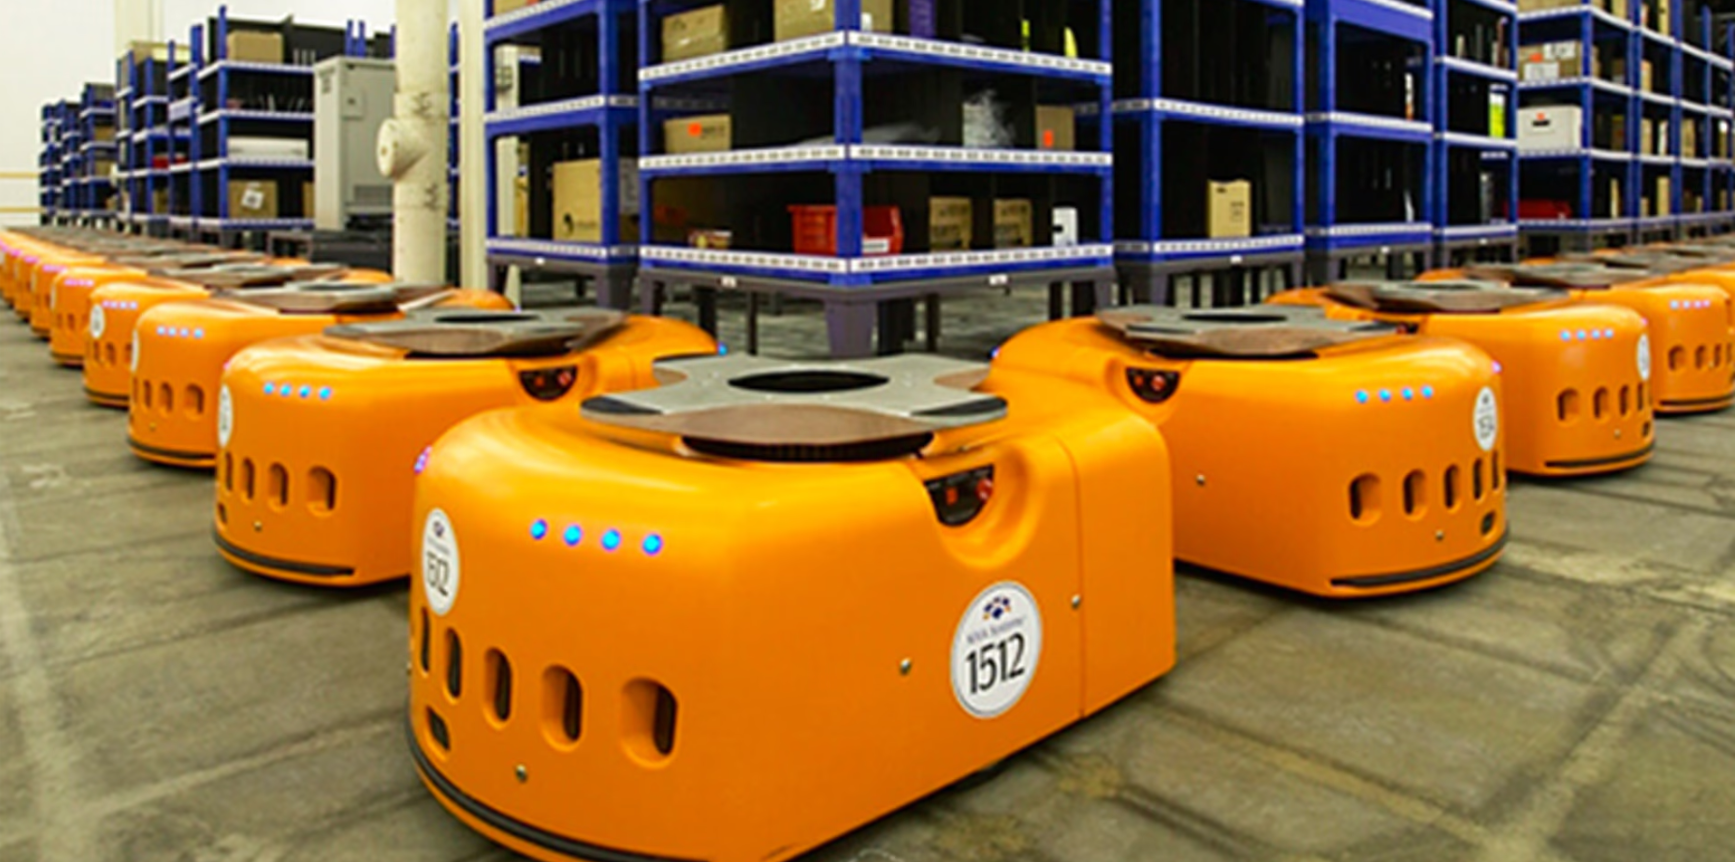
\includegraphics[width=\linewidth]{figures/Chapter 2/Amazon_kiva_robots.png}
        \caption{Amazon Kiva}
        \label{fig:kiva}
    \end{subfigure}
    
    \vspace{0.5cm}
    
    % Row 2: Geek+, Locus, AUSRA
    \begin{subfigure}[b]{0.3\textwidth}
        \centering
        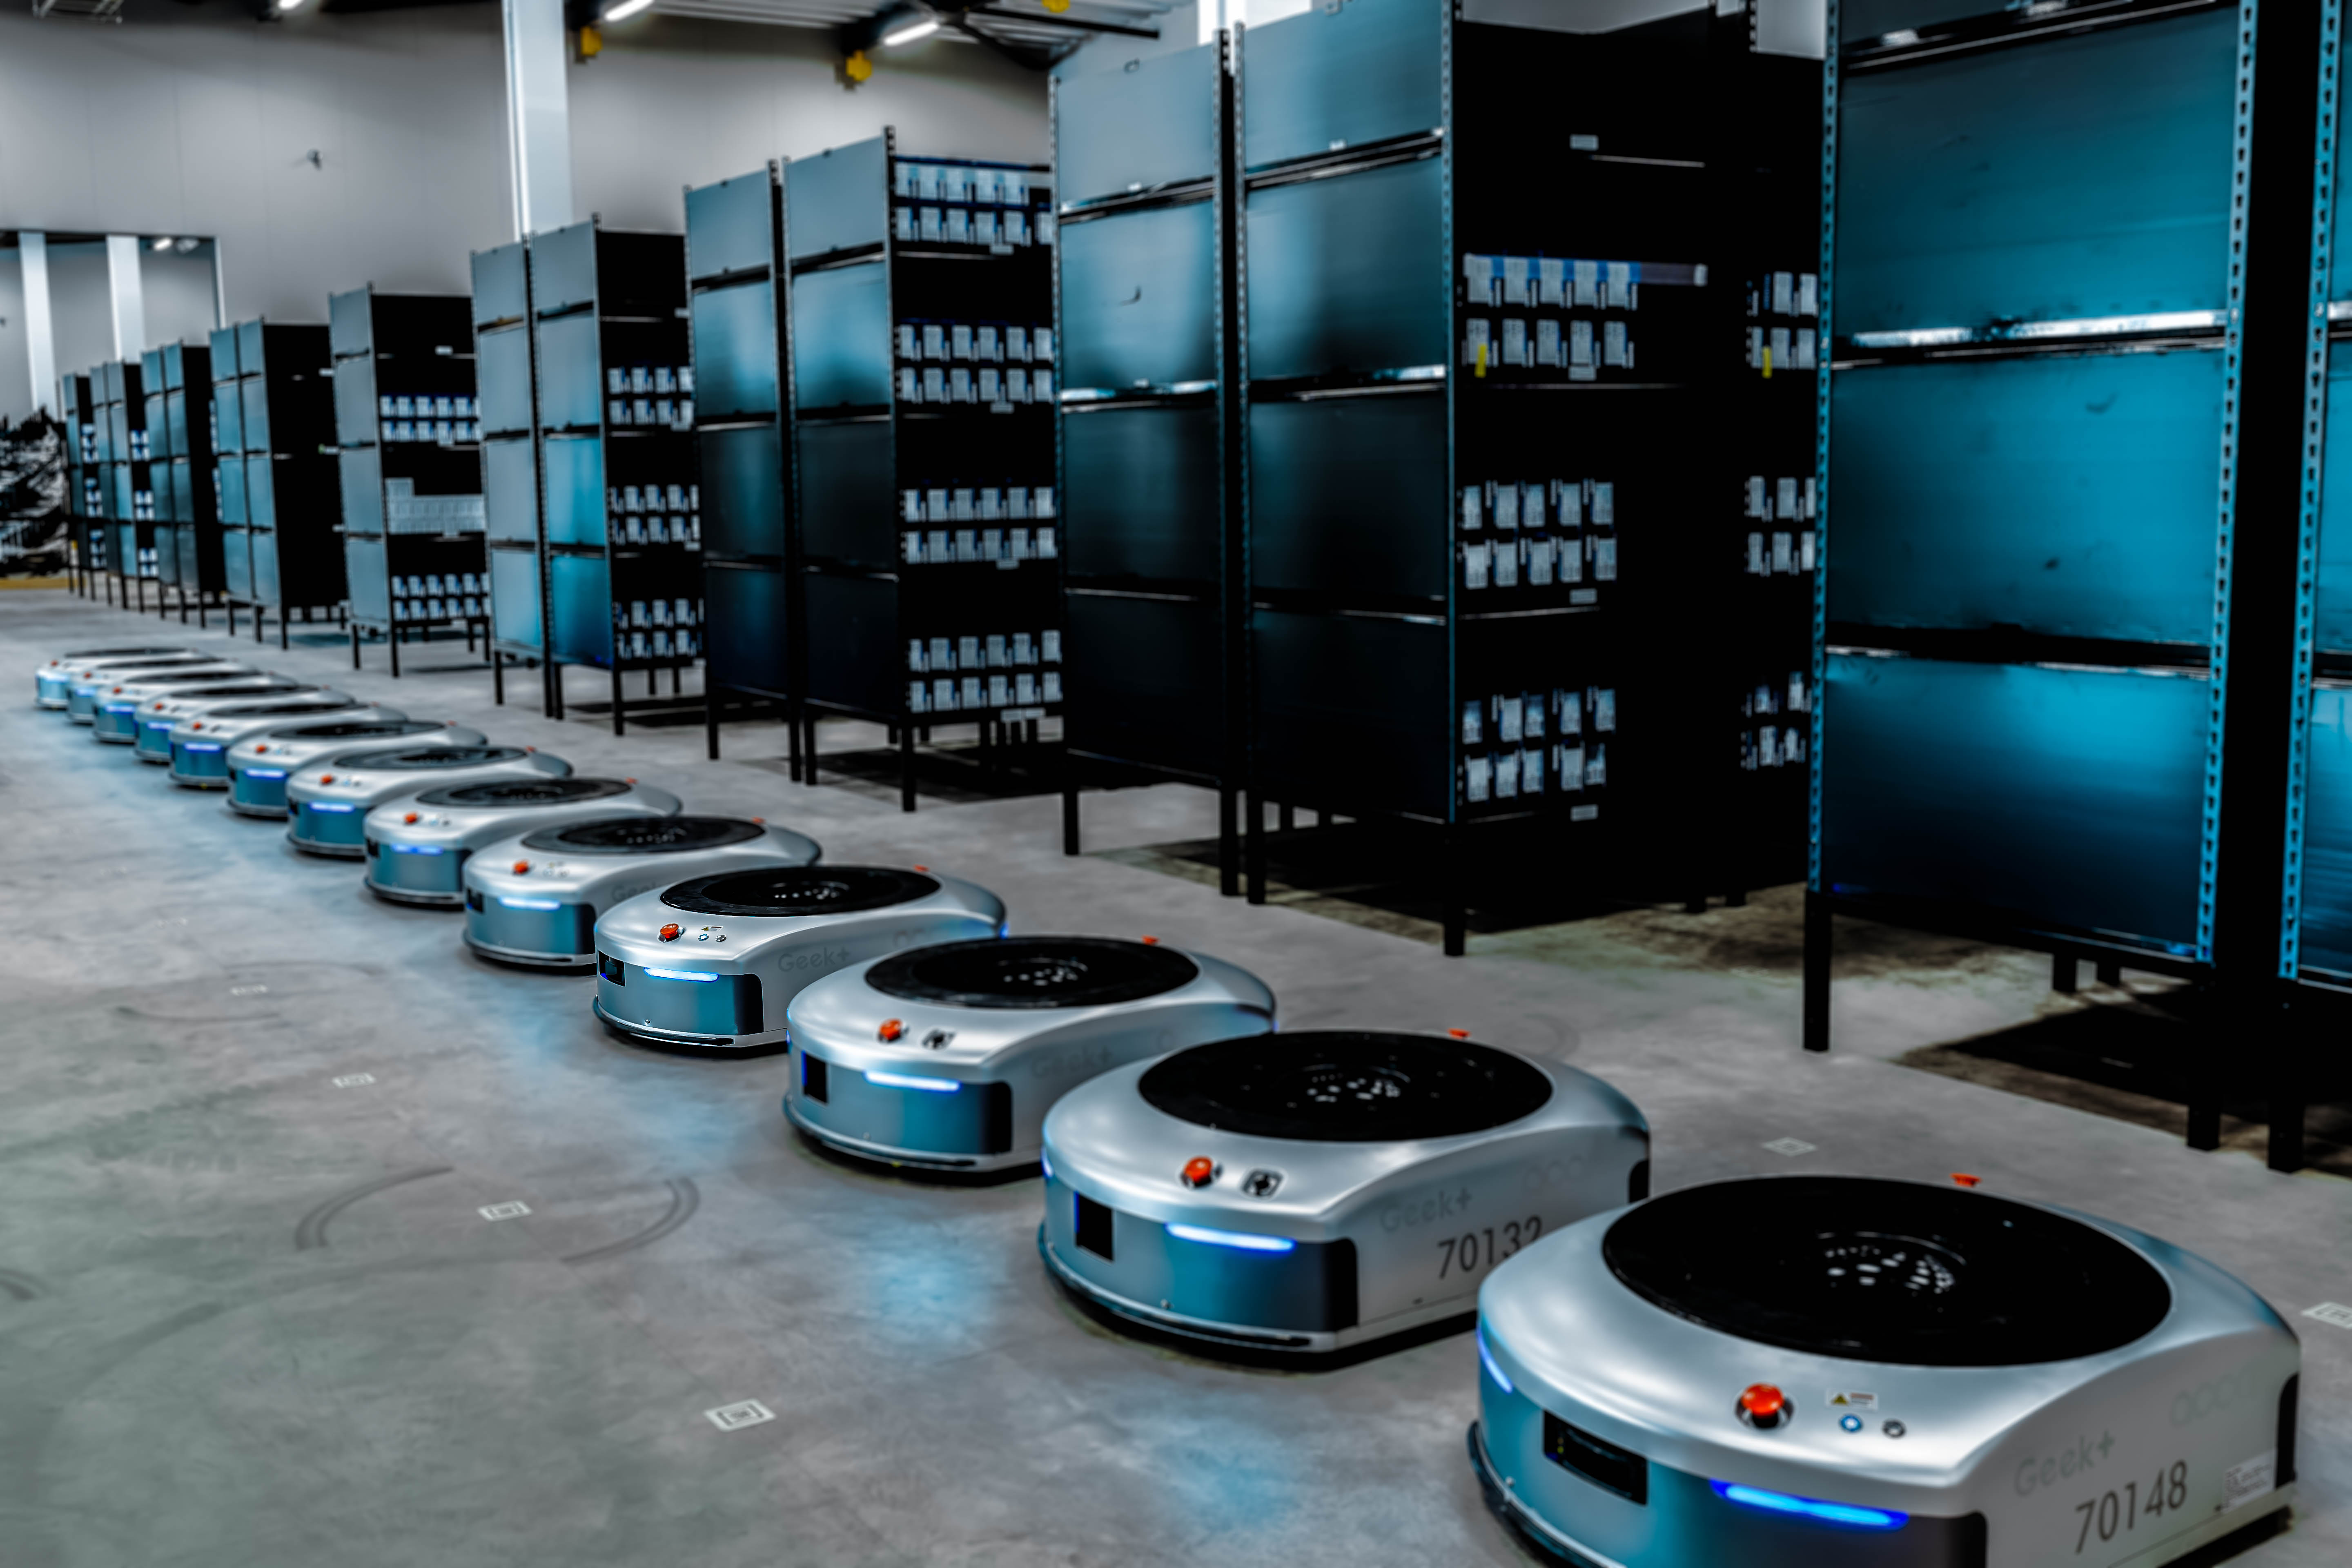
\includegraphics[width=\linewidth]{figures/Chapter 2/GeekPlus_robots.jpg}
        \caption{Geek+}
        \label{fig:geekplus}
    \end{subfigure}
    \hfill
    \begin{subfigure}[b]{0.3\textwidth}
        \centering
        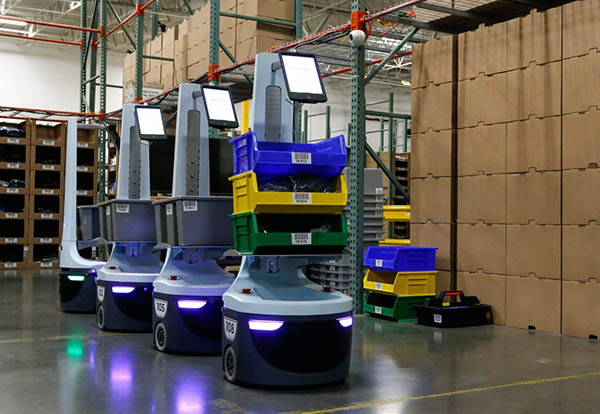
\includegraphics[width=\linewidth]{figures/Chapter 2/Locus_Bots.jpg}
        \caption{Locus Bots}
        \label{fig:locus}
    \end{subfigure}
    \hfill
    \begin{subfigure}[b]{0.3\textwidth}
        \centering
        \includegraphics[width=\linewidth]{figures/Chapter 2/Swarm_AUSRA.png}
        \caption{Our proposed AUSRA robot}
        \label{fig:ausra_proposed}
    \end{subfigure}
    
    \caption{Comparison of Existing Commercial/Research Robots and Proposed AUSRA Architecture}
    \label{fig:swarm_comparison}
\end{figure}
\newpage
\section{Mechanical Design Precedents}
\label{sec:mechanical_precedents}

\subsection{Chassis Design Approaches}
Previous research has explored various chassis configurations for mobile robots:

\begin{itemize}
    \item \textbf{Modular Designs:} Allow reconfiguration for different tasks
    \item \textbf{Monolithic Designs:} Provide structural integrity at the cost of flexibility
    \item \textbf{3D-Printed Prototypes:} Enable rapid iteration but may lack durability
\end{itemize}

\subsection{Material Selection Studies}
Material selection for mobile robot platforms typically considers:
\begin{itemize}
    \item Weight-to-strength ratio
    \item Cost and availability
    \item Manufacturability
    \item Environmental resistance
\end{itemize}

Common materials include aluminum alloys (6061-T6), ABS plastic, polycarbonate, and carbon fiber composites.

% Add your detailed content here...

\section{Control Strategies}
\label{sec:control_strategies}

\subsection{Centralized vs. Decentralized Approaches}

\textbf{Centralized Control:}
\begin{itemize}
    \item Single controller coordinates all robots
    \item Global optimization possible
    \item Single point of failure
    \item Communication bottleneck
\end{itemize}

\textbf{Decentralized Control:}
\begin{itemize}
    \item Each robot makes local decisions
    \item Scalable and robust
    \item Emergent global behavior
    \item Coordination challenges
\end{itemize}

\textbf{Hybrid Approaches:}
Modern systems often combine both paradigms:
\begin{itemize}
    \item Centralized task allocation with decentralized execution
    \item Hierarchical control structures
    \item Consensus-based decision making
\end{itemize}

\begin{figure}[H]
    \centering
    \includegraphics[width=\linewidth]{figures/Chapter 2/Centralized vs Decentralized vs Hybrid.png}
    \caption{Comparison of Control Architectures: Centralized vs. Decentralized vs. Hybrid}
    \label{fig:control_arch}
\end{figure}

\subsection{Navigation and Path Planning}
Key algorithms in multi-robot navigation include:
\begin{itemize}
    \item \textbf{A* and Dijkstra:} Global path planning
    \item \textbf{RRT/RRT*:} Sampling-based planning for complex spaces
    \item \textbf{DWA:} Dynamic Window Approach for local planning
    \item \textbf{VFH:} Vector Field Histogram for obstacle avoidance
\end{itemize}

% Add your detailed content here...

\section{Design Frameworks in Swarm Robotics}
\label{sec:design_frameworks}

Recent research has highlighted the need for structured frameworks to understand the complexity of designing robot swarms across different scales and contexts. Garzón Ramos \cite{garzonramos2024designing} proposes a three-level framework adapted from organizational theory that categorizes swarm design challenges as puzzles, problems, and the mess.

\subsection{The Puzzle: Understanding Self-Organization}
\label{subsec:puzzle}

At the foundational level, swarm robotics research has focused on \textbf{puzzles} --- well-defined scenarios where all information is available, the problem can be isolated, and repeatable solutions exist. Classic examples include:

\begin{itemize}
    \item \textbf{Aggregation:} Discovering rules that make robots cluster together
    \item \textbf{Flocking:} Identifying coordination mechanisms for collective motion
    \item \textbf{Pattern Formation:} Determining control laws for specific geometric arrangements
\end{itemize}

These studies establish the fundamental principles of self-organization and emergence in multi-robot systems. Once the underlying rules are discovered, they become generalizable primitives that can be reproduced across different platforms.

\subsection{The Problem: Task-Oriented Design with Trade-offs}
\label{subsec:problem}

As the field matures into an engineering discipline, the focus shifts to \textbf{problems} --- scenarios introducing uncertainty and multiple solutions with different trade-offs. At this level:

\begin{itemize}
    \item \textbf{Performance Metrics:} Designers must define what constitutes successful behavior
    \item \textbf{Automatic Design:} Optimization and machine learning methods combine self-organization primitives to achieve specific task objectives
    \item \textbf{Behavior Composition:} Finite state machines or behavior trees orchestrate different collective behaviors across mission phases
\end{itemize}

The AUSRA system operates primarily at this level, leveraging known principles of swarm coordination while optimizing for warehouse automation tasks. The architecture combines multiple behavioral primitives (navigation, collision avoidance, task allocation) with performance-driven tuning.

\subsection{The Mess: Real-World Deployment Complexity}
\label{subsec:mess}

The highest level of complexity represents \textbf{the mess} --- systems operating in real-world environments with:

\begin{itemize}
    \item \textbf{Human Interaction:} Workers, customers, and operators sharing the workspace
    \item \textbf{Uncontrolled Variables:} Dynamic obstacles, changing lighting, network disruptions
    \item \textbf{Interdependent Systems:} Integration with existing infrastructure and workflows
    \item \textbf{Context Awareness:} Understanding situational requirements beyond pre-programmed behaviors
\end{itemize}

Embracing "the mess" requires acknowledging that not all variables can be controlled or optimized. Future swarm systems must develop adaptive capabilities, robust failure modes, and intuitive human interfaces to operate reliably in these complex scenarios.

\subsection{Stigmergy as an Interface Mechanism}
\label{subsec:stigmergy}

\textbf{Stigmergy} --- communication through environmental modification --- offers a promising approach for bridging human-swarm interaction, particularly in manufacturing and logistics contexts \cite{garzonramos2024designing}. Unlike explicit digital communication, stigmergy allows:

\begin{itemize}
    \item \textbf{Implicit Coordination:} Objects placed in specific locations signal intent to nearby robots
    \item \textbf{Low-Bandwidth Interaction:} No need for Wi-Fi connectivity or complex user interfaces
    \item \textbf{Organic Integration:} Humans and robots share the same physical workspace naturally
\end{itemize}

For example, a worker placing a component in a designated area triggers robot pickup and transport without explicit commands. The environment itself becomes the communication medium, reducing cognitive load and system complexity.

\subsection{AUSRA's Position in the Framework}
\label{subsec:ausra_framework}

The AUSRA project addresses challenges at the \textbf{problem} level:
\begin{itemize}
    \item Combining navigation, localization, and coordination primitives
    \item Optimizing for task performance in structured warehouse environments
    \item Providing a modular architecture for different operational scenarios
\end{itemize}

While acknowledging the complexity of \textbf{the mess} as future work, AUSRA establishes a foundation for transitioning swarm research from controlled experiments to practical applications.



\section{Multi-Robot Exploration and Mapping}
\label{sec:mr_slam}

A critical component of collaborative swarm systems is the ability to enable multiple robots to simultaneously map an unknown environment and localize themselves within it. This problem, known as Multi-Robot SLAM (MR-SLAM), extends the traditional Simultaneous Localization and Mapping (SLAM) problem to distributed systems.

\subsection{Collaborative Mapping Approaches}
Early work by Simmons et al. \cite{simmons2000coordination} and Burgard et al. \cite{burgard2005coordinated} demonstrated that coordinating the exploration targets of multiple robots significantly reduces the time required to map a given area. The "frontier-based exploration" strategy proposed by Yamauchi \cite{yamauchi1997frontier} remains a foundational concept, where robots are directed to the boundaries between open space and unexplored territory.

More recently, sampling-based methods such as Rapidly-exploring Random Trees (RRTs) have been adapted for autonomous multi-robot exploration \cite{umari2017autonomous}, enabling efficient coverage of complex, cluttered environments.

\subsection{Greedy Frontier Exploration: \texttt{explore\_lite}}
\label{subsec:explore_lite}
A practical and widely-adopted realization of Yamauchi's frontier strategy is the open-source \texttt{explore\_lite} package from the \texttt{m-explore} stack \cite{hornerexplore}. Rather than maintaining an explicit map representation of its own, \texttt{explore\_lite} operates directly on the occupancy grid published by the navigation costmap, making it lightweight and straightforward to integrate with a Nav2-based stack. The node continuously detects frontiers --- contiguous boundaries between free and unknown cells --- and selects the next goal by ranking candidate frontiers with a weighted cost function that trades off the distance to a frontier against its size (information gain) and the robot's current heading. The selected frontier centroid is then dispatched as a navigation goal, and the cycle repeats until no frontiers remain, at which point the environment is considered fully explored.

The AUSRA system adopts \texttt{explore\_lite} as its single-robot exploration driver. Its frontier-ranking weights and detection thresholds were tuned for the cluttered indoor environments characteristic of search-and-rescue scenarios: the minimum frontier size was lowered so that narrow passages are not missed, the gain term was increased to favour expanding the mapped area, and the potential (distance) term was balanced to produce smoother transitions between successive frontiers rather than erratic back-and-forth motion. The specific parameter values and the tuning rationale are detailed in Chapter~\ref{chap:hardware}.

\subsection{Pose Graph Optimization}
Collaborative mapping often relies on a shared "Pose Graph" to maintain consistency across the swarm's global map. In this framework, each robot's trajectory is represented as a series of nodes (poses) connected by constraints derived from odometry and sensor measurements. A key challenge in MR-SLAM is "loop closure" --- recognizing when a robot has returned to a previously visited location or crossed paths with another robot. When a loop closure is detected, the entire graph is optimized to minimize error accumulation. Tools like SLAM Toolbox \cite{macenski2021slam} provide robust implementations of pose graph optimization that can be adapted for multi-robot scenarios, as demonstrated in the RoboSAR project.

\subsection{Multi-Robot Map Merging}
\label{subsec:map_merging}
Whereas pose graph optimization fuses observations \emph{within} a single robot's trajectory, a swarm tasked with collaboratively mapping an environment must additionally combine the individual occupancy grids produced by each agent into a single, globally consistent map. This fusion problem --- map merging --- can be approached in two fundamentally different ways.

The first approach, \textbf{feature-based merging}, makes no assumption about where the robots started. Instead, it treats each robot's map as an image and searches for the rigid transformation (rotation and translation) that best aligns overlapping structure, typically by extracting and matching visual features between the grids. This is robust to unknown starting configurations but depends on the maps sharing enough overlapping, distinctive geometry for a confident match, and it can fail or produce misaligned results in featureless or highly symmetric spaces.

The second approach, \textbf{merging from known initial poses}, assumes the relative spawn positions of the robots are known in advance. Each map can then be transformed directly into a common world frame using the known offsets, sidestepping the feature-matching step entirely and guaranteeing a deterministic, correctly-scaled merge. The trade-off is the operational requirement that robots be deployed from surveyed or otherwise known starting points.

The open-source \texttt{multirobot\_map\_merge} package, also part of the \texttt{m-explore} stack \cite{hornerexplore}, implements both strategies and is selectable at runtime via a single parameter. The AUSRA system adopts the \textbf{known-initial-pose} strategy: in a coordinated search-and-rescue deployment the robots are launched from a known formation, so their relative offsets are available and a deterministic merge is preferable to the uncertainty of feature matching on the sparse grids typical of partially-explored disaster environments. The concrete realization of this strategy on the AUSRA hardware --- including how each robot's spawn offset is incorporated and how the per-robot maps are aggregated into a shared global map --- is presented in Chapter~\ref{chap:swarm}.

\section{Task Allocation in Swarms}
\label{sec:task_allocation}

Efficiently assigning tasks to individual robots is essential for maximizing the performance of a swarm. Korsah et al. \cite{korsah2013comprehensive} provide a comprehensive taxonomy for Multi-Robot Task Allocation (MRTA), categorizing problems based on:
\begin{itemize}
    \item \textbf{Single-Task vs. Multi-Task Robots (ST/MT):} Whether a robot can perform one or multiple tasks at a time.
    \item \textbf{Single-Robot vs. Multi-Robot Tasks (SR/MR):} Whether a task requires one or multiple robots to complete.
    \item \textbf{Instantaneous vs. Time-Extended Assignment (IA/TA):} Whether tasks are assigned immediately or planned over a future horizon.
\end{itemize}

\begin{figure}[H]
    \centering
    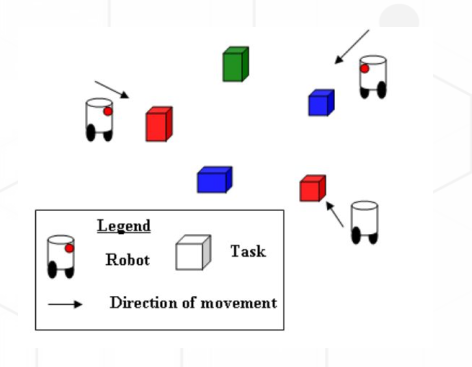
\includegraphics[width=0.6\linewidth]{figures/Chapter 2/Task_allocation.png}
    \caption{Taxonomy of Multi-Robot Task Allocation (MRTA)}
    \label{fig:task_allocation}
\end{figure}

For Search and Rescue (SAR) applications, Queralta et al. \cite{queralta2020collaborative} highlight the importance of dynamic task allocation mechanisms that can adapt to the changing state of the environment and the swarm, such as the discovery of a victim or the failure of a robot agent.

\section{Summary}
\label{sec:lit_summary}

This literature review has identified key considerations for the AUSRA system:
\begin{enumerate}
    \item A hybrid control architecture balances scalability and coordination
    \item Omnidirectional locomotion offers superior maneuverability for swarm operations
    \item Modular mechanical design enables flexibility and maintainability
    \item ROS provides a robust framework for autonomous navigation
\end{enumerate}

The following chapters detail how these insights informed the design and implementation of the AUSRA system.
